\documentclass[11pt,a4paper,addpoints]{exam}
\usepackage[utf8]{inputenc}
\usepackage[T1]{fontenc}
\usepackage{lmodern}
\usepackage{amsmath,amssymb}
\usepackage[a4paper,margin=2cm]{geometry}
\usepackage{siunitx}
\sisetup{output-decimal-marker={,},per-mode=symbol,group-separator={.}}
\usepackage{tikz}
\usetikzlibrary{arrows.meta,decorations.markings,patterns}
\usepackage[american]{circuitikz}
\usepackage{xcolor}

% ---- localização do pacote exam ----
\pointpoints{ponto}{pontos}
\qformat{\textbf{Questão \thequestion}\quad\textit{(\totalpoints\ pts)}\hfill}
\renewcommand{\partlabel}{(\thepartno)}
\renewcommand{\solutiontitle}{\noindent\textbf{Solução:}\enspace}
\hqword{Questão}\hpword{Pontos}\hsword{Nota}\htword{Total}

\pagestyle{headandfoot}
\firstpageheader{}{}{}
\runningheader{\small Física Geral III — Avaliação}{}{\small IFES — Campus Vitória}
\footer{}{\small Página \thepage\ de \numpages}{}
\runningheadrule

\newcommand{\vu}[1]{\hat{\boldsymbol{#1}}}

\begin{document}

\begin{center}
  {\large\textbf{INSTITUTO FEDERAL DO ESPÍRITO SANTO — CAMPUS VITÓRIA}}\\[2pt]
  Coordenadoria de Física\\[6pt]
  {\Large\textbf{Física Geral III — Eletromagnetismo}}\\[2pt]
  {\large Avaliação: Campo magnético, indução e circuitos RLC}
\end{center}

\vspace{4pt}
\noindent\makebox[0.68\textwidth]{Nome:\enspace\hrulefill}\hfill
\makebox[0.28\textwidth]{Turma:\enspace\hrulefill}\\[8pt]
\noindent\makebox[0.48\textwidth]{Professor: Célio Marques}\hfill
\makebox[0.48\textwidth]{Data:\enspace\hrulefill}

\vspace{6pt}
\begin{center}
\gradetable[h][questions]
\end{center}

\noindent\fbox{\parbox{\dimexpr\textwidth-2\fboxsep-2\fboxrule}{\small
\textbf{Instruções.} (i) Resolva cada questão de forma organizada: parta das leis físicas, justifique as aproximações e só substitua números no final. (ii) Respostas numéricas sem desenvolvimento não serão consideradas. (iii) Use $\mu_0 = 4\pi\times10^{-7}\ \si{T.m/A}$. (iv) É permitido o uso de calculadora científica. (v) Duração: 100 minutos. (vi) Pontuação total: 100 pontos; nota $=$ pontos$/10$. Um formulário encontra-se na última página.}}

\begin{questions}

% =====================================================================
\question
\textbf{Lei de Biot–Savart.} Uma espira circular de raio $a = \SI{10,0}{cm}$ conduz uma corrente estacionária $I = \SI{5,0}{A}$.

\begin{parts}
\part[8] Partindo da lei de Biot–Savart,
$d\vec B = \dfrac{\mu_0}{4\pi}\dfrac{I\,d\vec\ell\times\vu{r}}{r^2}$,
mostre que o campo em um ponto do eixo da espira, a uma distância $z$ do seu centro, é
\[
  B(z) = \frac{\mu_0 I a^2}{2\left(a^2+z^2\right)^{3/2}}.
\]
Explique, com argumento de simetria, por que as componentes de $d\vec B$ perpendiculares ao eixo se cancelam.
\part[4] Calcule o módulo do campo no centro da espira e em $z = \SI{10,0}{cm}$.
\part[5] A mesma corrente percorre agora uma espira \emph{quadrada} de lado $L = \SI{20,0}{cm}$. Sabendo que um segmento retilíneo finito produz, a uma distância perpendicular $d$, o campo $B = \dfrac{\mu_0 I}{4\pi d}\left(\sin\theta_2 - \sin\theta_1\right)$, mostre que no centro do quadrado
$B_{\square} = \dfrac{2\sqrt2\,\mu_0 I}{\pi L}$ e calcule-o. Compare com o campo no centro de uma espira circular \emph{inscrita} no quadrado ($a = L/2$) e interprete a diferença.
\part[3] Mostre que, para $z \gg a$, o campo no eixo se reduz a $B \approx \dfrac{\mu_0\, \mathfrak{m}}{2\pi z^3}$, com $\mathfrak{m} = I\pi a^2$. Qual o significado físico de $\mathfrak{m}$?
\end{parts}

% =====================================================================
\question
\textbf{Lei de Faraday.} Um fio retilíneo muito longo conduz a corrente $I = \SI{20}{A}$. Uma espira retangular, coplanar ao fio, tem lados $\ell = \SI{20}{cm}$ (paralelo ao fio) e $w = \SI{10}{cm}$ (perpendicular ao fio), e resistência $R = \SI{0,010}{\ohm}$. O lado mais próximo do fio está à distância $x$ (figura).

\begin{center}
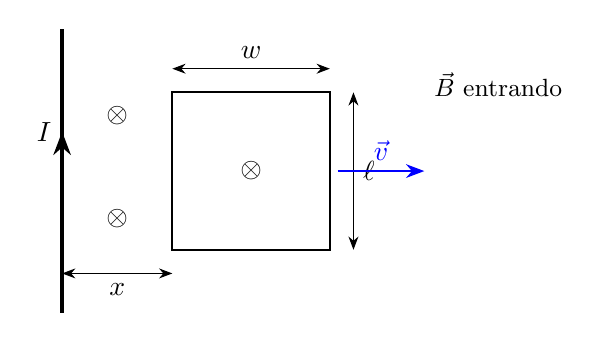
\begin{tikzpicture}[scale=1.0,>=Stealth]
  \draw[very thick] (0,-0.3) -- (0,3.3);
  \draw[->,very thick] (0,1.2) -- (0,2.0) node[left]{$I$};
  \draw[thick] (1.4,0.5) rectangle (3.4,2.5);
  \draw[<->] (0,0.2) -- node[below]{$x$} (1.4,0.2);
  \draw[<->] (1.4,2.8) -- node[above]{$w$} (3.4,2.8);
  \draw[<->] (3.7,0.5) -- node[right]{$\ell$} (3.7,2.5);
  \draw[->,thick,blue] (3.5,1.5) -- node[above]{$\vec v$} (4.6,1.5);
  \foreach \p in {(0.7,0.9),(0.7,2.2),(2.4,1.5)} \node at \p {$\otimes$};
  \node[right] at (4.6,2.6) {\small $\vec B$ entrando};
\end{tikzpicture}
\end{center}

\begin{parts}
\part[5] Mostre que o fluxo magnético através da espira é
$\Phi_B(x) = \dfrac{\mu_0 I \ell}{2\pi}\ln\!\left(\dfrac{x+w}{x}\right)$.
\part[6] A espira se afasta do fio com velocidade constante $v = \SI{2,0}{m/s}$. Determine a fem induzida e a corrente induzida no instante em que $x = \SI{5,0}{cm}$. Indique o sentido da corrente (horário ou anti-horário, na figura), justificando pela lei de Lenz.
\part[4] Confirme o resultado do item (b) calculando a fem de movimento $\oint(\vec v\times\vec B)\cdot d\vec\ell$. Por que os lados perpendiculares ao fio não contribuem?
\part[5] Suponha agora a espira \emph{parada} em $x = \SI{5,0}{cm}$ e a corrente do fio alternada, $I(t) = I_0\sin(\omega t)$, com $I_0 = \SI{20}{A}$ e $f = \SI{60}{Hz}$. Obtenha $\varepsilon(t)$ e sua amplitude. Qual a defasagem entre $\varepsilon(t)$ e $I(t)$?
\end{parts}

% =====================================================================
\question
\textbf{Indutância mútua entre espiras concêntricas.} Duas espiras circulares coplanares e concêntricas têm raios $R_1 = \SI{20}{cm}$ e $R_2 = \SI{2,0}{cm}$ ($R_1 \gg R_2$). A espira maior tem uma volta e conduz $i_1(t) = I_0\sin(\omega t)$, com $I_0 = \SI{3,0}{A}$ e $f = \SI{1,0}{kHz}$. A espira menor é, na verdade, uma pequena bobina de $N_2 = 50$ voltas, com resistência $R = \SI{0,50}{\ohm}$ e autoindutância $L_2 = \SI{0,25}{mH}$, fechada sobre si mesma.

\begin{center}
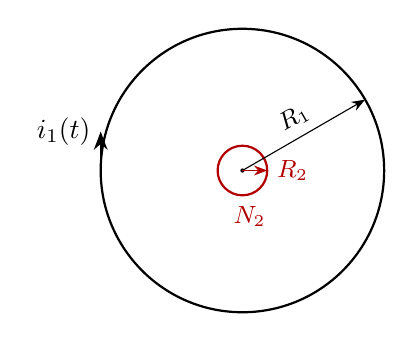
\begin{tikzpicture}[scale=0.9,>=Stealth]
  \draw[thick] (0,0) circle (2);
  \draw[thick,red!70!black] (0,0) circle (0.35);
  \fill (0,0) circle (0.03);
  \draw[->] (0,0) -- node[above,sloped]{\small $R_1$} (1.73,1.0);
  \draw[->,red!70!black] (0,0) -- (0.35,0) node[right]{\small $R_2$};
  \draw[->,thick] (-2,0.15) -- (-2,0.55) node[left]{$i_1(t)$};
  \node[red!70!black] at (0.1,-0.65) {\small $N_2$};
\end{tikzpicture}
\end{center}

\begin{parts}
\part[5] Justifique por que, para $R_2 \ll R_1$, o campo de $i_1$ pode ser considerado uniforme sobre a área da espira menor e mostre que
$M \approx \dfrac{\mu_0 \pi N_2 R_2^2}{2R_1}$. Calcule $M$.
\part[5] Obtenha a fem induzida $\varepsilon_2(t)$ na bobina menor e calcule sua amplitude.
\part[6] Determine a amplitude da corrente induzida $i_2(t)$ e o atraso de fase de $i_2$ em relação a $\varepsilon_2$. É razoável desprezar $L_2$ neste caso? Justifique numericamente.
\part[4] Se, em vez disso, a corrente $I_0\sin(\omega t)$ circulasse na bobina menor, qual seria a amplitude da fem induzida na espira maior? Por que calcular essa situação \emph{diretamente} (pelo fluxo através da espira grande) seria muito mais trabalhoso?
\end{parts}

% =====================================================================
\question
\textbf{Circuito RLC série.} Um circuito RLC série tem $R = \SI{20}{\ohm}$, $L = \SI{50}{mH}$ e $C = \SI{2,0}{\micro F}$, alimentado por uma fonte senoidal de amplitude $V_0 = \SI{10}{V}$ e frequência ajustável.

\begin{center}
\begin{circuitikz}[scale=0.85, transform shape]
  \draw (0,0) to[sV, l=$v(t)$] (0,3)
        to[R, l=$R$] (3,3)
        to[L, l=$L$] (6,3)
        to[C, l=$C$] (6,0) -- (0,0);
\end{circuitikz}
\end{center}

\begin{parts}
\part[5] Calcule a frequência de ressonância $f_0$, o fator de qualidade $Q$ e a largura de banda $\Delta f$ (meia potência).
\part[5] Na ressonância, calcule a amplitude da corrente, a potência média dissipada e a amplitude da tensão no indutor. Comente o fato de $V_L$ ser muito maior que $V_0$: isso viola a conservação de energia?
\part[6] Para $f = \SI{400}{Hz}$, calcule a impedância, a amplitude da corrente, o ângulo de fase $\phi$ entre a tensão da fonte e a corrente e a potência média. O circuito é predominantemente capacitivo ou indutivo?
\part[4] A fonte é removida com o capacitor carregado a $\SI{10}{V}$ e o circuito RLC é fechado sobre si mesmo. Classifique o regime (sub, super ou criticamente amortecido), calcule a frequência angular das oscilações amortecidas, o valor de $R$ que tornaria o amortecimento crítico e o tempo para a amplitude da carga cair a $1/e$ do valor inicial.
\end{parts}

% =====================================================================
\question
\textbf{Aplicação: como funciona um alto-falante (ou fone de ouvido)?} Num alto-falante dinâmico, uma bobina móvel presa ao cone fica no entreferro de um ímã permanente, onde o campo é \emph{radial}. Considere: fator de força $B\ell = \SI{7,0}{T.m}$ ($\ell$ é o comprimento total de fio imerso no campo), resistência da bobina $R_e = \SI{6,0}{\ohm}$, indutância da bobina $L_e = \SI{0,50}{mH}$, massa móvel $m = \SI{20}{g}$, rigidez da suspensão $k = \SI{2,0e3}{N/m}$ e amortecimento mecânico $b = \SI{1,5}{N.s/m}$.

\begin{center}
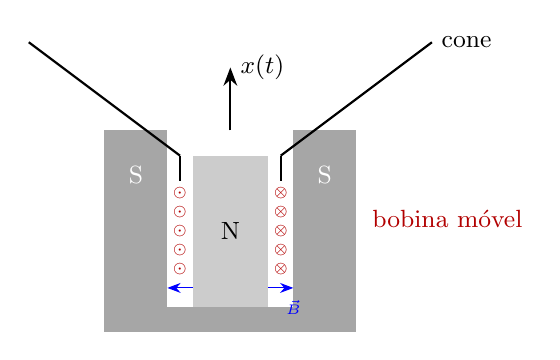
\begin{tikzpicture}[scale=0.8,>=Stealth]
  % ímã
  \fill[gray!40] (-0.6,-1.2) rectangle (0.6,1.2);
  \node at (0,0) {\small N};
  \fill[gray!70] (-2.0,-1.6) rectangle (-1.0,1.6);
  \fill[gray!70] (1.0,-1.6) rectangle (2.0,1.6);
  \fill[gray!70] (-2.0,-1.6) rectangle (2.0,-1.2);
  \node[white] at (-1.5,0.9) {\small S}; \node[white] at (1.5,0.9) {\small S};
  % bobina
  \foreach \y in {-0.6,-0.3,0,0.3,0.6} { \node[red!70!black] at (-0.8,\y) {\tiny$\odot$}; \node[red!70!black] at (0.8,\y) {\tiny$\otimes$}; }
  \draw[->,blue] (0.6,-0.9) -- (1.0,-0.9); \draw[->,blue] (-0.6,-0.9) -- (-1.0,-0.9);
  \node[blue,below] at (1.0,-0.95) {\tiny $\vec B$};
  % cone
  \draw[thick] (-0.8,1.2) -- (-3.2,3.0); \draw[thick] (0.8,1.2) -- (3.2,3.0);
  \draw[thick] (-0.8,1.2) -- (-0.8,0.8); \draw[thick] (0.8,1.2) -- (0.8,0.8);
  \draw[->,thick] (0,1.6) -- (0,2.6) node[right]{\small $x(t)$};
  \node[right] at (3.2,3.0) {\small cone};
  \node[right,red!70!black] at (2.1,0.2) {\small bobina móvel};
\end{tikzpicture}
\end{center}

\begin{parts}
\part[4] Explique, passo a passo, como um sinal elétrico de áudio se transforma em som. Por que o campo no entreferro é projetado para ser radial?
\part[4] Quando o cone se move com velocidade $v$, a lei de Faraday prevê uma fem induzida na bobina. Mostre que $\varepsilon = B\ell\, v$ e calcule-a para $v = \SI{0,50}{m/s}$. Pela lei de Lenz, essa fem auxilia ou se opõe à corrente que move o cone?
\part[6] Escreva a equação mecânica do cone, $m\ddot x + b\dot x + kx = B\ell\, i$, e a equação do circuito, $V = R_e i + L_e \dfrac{di}{dt} + B\ell\,\dot x$. Mostre que, vista pelo amplificador, a parte mecânica equivale a um \textbf{circuito RLC paralelo} com
\[
  C_{\text{eq}} = \frac{m}{(B\ell)^2},\qquad L_{\text{eq}} = \frac{(B\ell)^2}{k},\qquad R_{\text{eq}} = \frac{(B\ell)^2}{b},
\]
em série com $R_e$ e $L_e$. Calcule $C_{\text{eq}}$, $L_{\text{eq}}$ e $R_{\text{eq}}$.
\part[4] Calcule a frequência de ressonância $f_s$ e o módulo da impedância elétrica nessa frequência. Por que a curva $|Z(f)|$ de um alto-falante apresenta um pico, e não um vale, em $f_s$?
\part[2] Explique por que um fone de ouvido dinâmico, ligado à entrada de microfone de um computador, funciona como microfone.
\end{parts}

\end{questions}

\newpage
\begin{center}\large\textbf{Formulário}\end{center}
\small
\begin{align*}
&d\vec B = \frac{\mu_0}{4\pi}\frac{I\,d\vec\ell\times\vu r}{r^2}
&&B_{\text{fio longo}} = \frac{\mu_0 I}{2\pi r}
&&B_{\text{segmento}} = \frac{\mu_0 I}{4\pi d}(\sin\theta_2-\sin\theta_1)\\[4pt]
&\varepsilon = -\frac{d\Phi_B}{dt},\quad \Phi_B = \int \vec B\cdot d\vec A
&&\varepsilon_{\text{mov}} = \oint (\vec v\times\vec B)\cdot d\vec\ell
&&\Phi_{21} = M i_1,\quad \varepsilon_2 = -M\frac{di_1}{dt}\\[4pt]
&X_L = \omega L,\quad X_C = \frac{1}{\omega C}
&&Z = \sqrt{R^2 + (X_L-X_C)^2}
&&\tan\phi = \frac{X_L - X_C}{R}\\[4pt]
&\omega_0 = \frac{1}{\sqrt{LC}},\quad Q = \frac{\omega_0 L}{R},\quad \Delta\omega = \frac{R}{L}
&&P_{\text{méd}} = \tfrac12 I_0^2 R
&&\alpha = \frac{R}{2L},\quad \omega_d = \sqrt{\omega_0^2-\alpha^2}\\[4pt]
&\vec F = I\,\vec\ell\times\vec B
&&\int\frac{dx}{x} = \ln x
&&(1+u)^{-3/2}\approx 1-\tfrac32 u\ \ (u\ll1)
\end{align*}

\vfill
\begin{center}\footnotesize
Gabarito comentado e interativo: aplicativo Streamlit \texttt{avaliacao-fg3} (link no GitHub da disciplina).
\end{center}

\end{document}
